\chapter{الماء والجزيئات الحيوية الصغيرة}\label{ch:b1:water-small-molecules}

بكتيريا حجمها ميكرومتر مكعب واحد تحوي نحو عشرين مليار جزيء ماء وبضع
مئات الملايين من كل ما عداه. والماء ليس خلفية \omterm{def:b1:cell-unit-of-life:cell}{الخلية} بل وسطها: فهو
يذيب الشوارد والسكريات، ويخفي الأجزاء الزيتية من البروتينات
\omterm{def:b1:membranes-transport:membrane}{والأغشية}، ويضبط الحموضة التي يتوقف عليها كل إنزيم، وهو متفاعل أو
ناتج في نصف تفاعلات الاستقلاب. يصف هذا الفصل الماء والروابط الضعيفة
التي يعقدها ويحلها، وحساب الحموض والأسس والهوادئ، والجزيئات العضوية
الصغيرة التي تُبنى منها جزيئات الفصول الأربعة التالية الكبيرة، \omterm{def:b1:water-small-molecules:atp}{وعملة
الطاقة} --- \omterm{def:b1:water-small-molecules:atp}{ATP} --- التي تدفع بها \omterm{def:b1:cell-unit-of-life:cell}{الخلية} ثمن بنائها.

\section{الماء}

\begin{definition}[جزيء الماء]\label{def:b1:water-small-molecules:water}
\index{ماء}
الماء، $\mathrm{H_2O}$، جزيء منحن (زاوية H--O--H فيه
$104.5^\circ$) يجذب فيه الأكسجين الإلكترونات المشتركة نحو نفسه: فهو
\emph{قطبي}\index{جزيء قطبي}، بشحنة سالبة جزئية على الأكسجين وشحنتين
موجبتين جزئيتين على الهيدروجينين. ويستطيع كل جزيء أن يعقد حتى أربع
\emph{روابط هيدروجينية}\index{رابطة هيدروجينية} --- وهي تجاذب
كهرساكن بين هيدروجين مرتبط بذرة كهرسلبية (O، N) وزوج إلكتروني حر على
ذرة كهرسلبية أخرى --- اثنتين عبر هيدروجينيه واثنتين عبر أكسجينه.
والماء السائل شبكة من هذه الروابط، عمر كل منها بضعة بيكوثوان.
\end{definition}

\begin{omfigure}
\begin{tikzpicture}[font=\small, line cap=round,
  O/.style={circle, draw, thick, fill=omThm!30, minimum size=8mm, inner sep=0pt},
  H/.style={circle, draw, thick, fill=gray!15, minimum size=5.5mm, inner sep=0pt}]
  % central water molecule
  \node[O] (O) at (0,0) {O};
  \node[H] (H1) at (-0.8,-0.7) {H};
  \node[H] (H2) at (0.8,-0.7) {H};
  \draw[thick] (O) -- (H1); \draw[thick] (O) -- (H2);
  \node[font=\scriptsize, omThm] at (0,0.62) {$\delta^-$};
  \node[font=\scriptsize] at (-1.4,-0.55) {$\delta^+$};
  \node[font=\scriptsize] at (1.4,-0.55) {$\delta^+$};
  % lower-left neighbour (accepts an H bond from H1)
  \node[O] (O2) at (-2.1,-2.3) {O};
  \node[H] (H2a) at (-3.05,-2.55) {H};
  \node[H] (H2b) at (-1.75,-3.3) {H};
  \draw[thick] (O2) -- (H2a); \draw[thick] (O2) -- (H2b);
  \draw[dashed, thick, omDef] (H1) -- (O2);
  % lower-right neighbour
  \node[O] (O3) at (2.1,-2.3) {O};
  \node[H] (H3a) at (3.05,-2.55) {H};
  \node[H] (H3b) at (1.75,-3.3) {H};
  \draw[thick] (O3) -- (H3a); \draw[thick] (O3) -- (H3b);
  \draw[dashed, thick, omDef] (H2) -- (O3);
  % upper-left neighbour (donates an H bond to O)
  \node[H] (H4) at (-1.1,1.55) {H};
  \node[O] (O4) at (-2.0,2.25) {O};
  \node[H] (H4b) at (-2.95,2.6) {H};
  \draw[thick] (O4) -- (H4); \draw[thick] (O4) -- (H4b);
  \draw[dashed, thick, omDef] (H4) -- (O);
  % upper-right neighbour
  \node[H] (H5) at (1.1,1.55) {H};
  \node[O] (O5) at (2.0,2.25) {O};
  \node[H] (H5b) at (2.95,2.6) {H};
  \draw[thick] (O5) -- (H5); \draw[thick] (O5) -- (H5b);
  \draw[dashed, thick, omDef] (H5) -- (O);
  \node[anchor=west, align=left, font=\footnotesize] at (4.0,1.0) {المتقطع: روابط هيدروجينية\\ (\qty{0.18}{nm}، ونحو \qty{20}{kJ/mol} لكل منها)\\ المتصل: روابط تساهمية O--H\\ (\qty{0.096}{nm}، \qty{460}{kJ/mol})};
  \node[anchor=west, align=left, font=\footnotesize] at (4.0,-1.3) {كل جزيء يمنح رابطتين\\ هيدروجينيتين ويقبل رابطتين:\\ فتنشأ شبكة رباعية السطوح};
\end{tikzpicture}

{\small جزيء ماء (زاوية H--O--H فيه $104.5^\circ$) وجيرانه الأربعة
المرتبطون به \omterm{def:b1:water-small-molecules:water}{بروابط هيدروجينية}. الجزيء المنحني \omterm{def:b1:water-small-molecules:water}{القطبي} يمنح رابطتين هيدروجينيتين
عبر هيدروجينيه ويقبل رابطتين على أكسجينه؛ والشبكة التي تكوّنانها تمنح
الماء تماسكه وسعته الحرارية وقوته مذيبًا.}
\end{omfigure}

\begin{proposition}[خواص الماء التي تهم الحياة]\label{prop:b1:water-small-molecules:properties}
تفسر شبكة \omterm{def:b1:water-small-molecules:water}{الروابط الهيدروجينية} خواص الماء الاستثنائية:
\begin{itemize}
  \item \emph{تماسك} عالٍ وتوتر سطحي عالٍ (\qty{72}{mN/m}): فأعمدة
        الماء يمكن أن تُسحب إلى أعلى شجرة دون أن تنقطع
        (\cref{ch:b1:plant-transport})؛ والحشرات تمشي على البرك؛
  \item \emph{سعة حرارية} عالية (\qty{4.18}{kJ.kg^{-1}.K^{-1}})
        وحرارة تبخر عالية (\qty{2.4}{kJ/g}): فحرارة \omterm{def:b1:organism-environment:organism}{الكائنات} الحية
        والمسطحات المائية تتغير ببطء، وتبخير غرام من العرق ينزع
        \qty{2.4}{kJ}؛
  \item \emph{صلب أقل كثافة من السائل}: فالجليد يطفو، والبحيرات تتجمد
        من أعلى إلى أسفل، فيبقى ماء سائل تحته؛
  \item \emph{مذيب} ممتاز للشوارد والجزيئات القطبية، إذ يحيطها بأغلفة
        موجهة (\emph{إماهة})، ومذيب رديء للجزيئات غير القطبية، إذ
        يجبرها على التجمع (\emph{الأثر الكاره للماء}\index{الأثر الكاره للماء}).
\end{itemize}
\end{proposition}
\begin{proof}[برهان جزئي]
التماسك والتوتر السطحي يقيسان شغل فصل جزيئات يمسك كلًا منها أربع
روابط قدر كل منها \qty{20}{kJ/mol}. وتسخين الماء يقتضي كسر الروابط
مع تحريك الجزيئات، ومن هنا السعة الحرارية؛ وتبخيره يقتضي كسرها
جميعًا. والجليد يمسك كل جزيء في شبكة رباعية السطوح مفتوحة من أربع
روابط، وهي تشغل حجمًا أكبر من السائل المضطرب الذي ترتص فيه الجزيئات
ارتصاصًا أكثف. والشوارد والزمر القطبية تستقر \omterm{def:b1:water-small-molecules:water}{بروابط هيدروجينية} مع
الماء؛ أما الجزيء غير \omterm{def:b1:water-small-molecules:water}{القطبي} فلا يستطيع عقدها، وعلى الماء حوله أن
ينتظم في قفص، بكلفة في الإنتروبيا تقل حين تتجمع الجزيئات غير القطبية
وتتقاسم قفصًا واحدًا.
\end{proof}

\begin{omfigure}
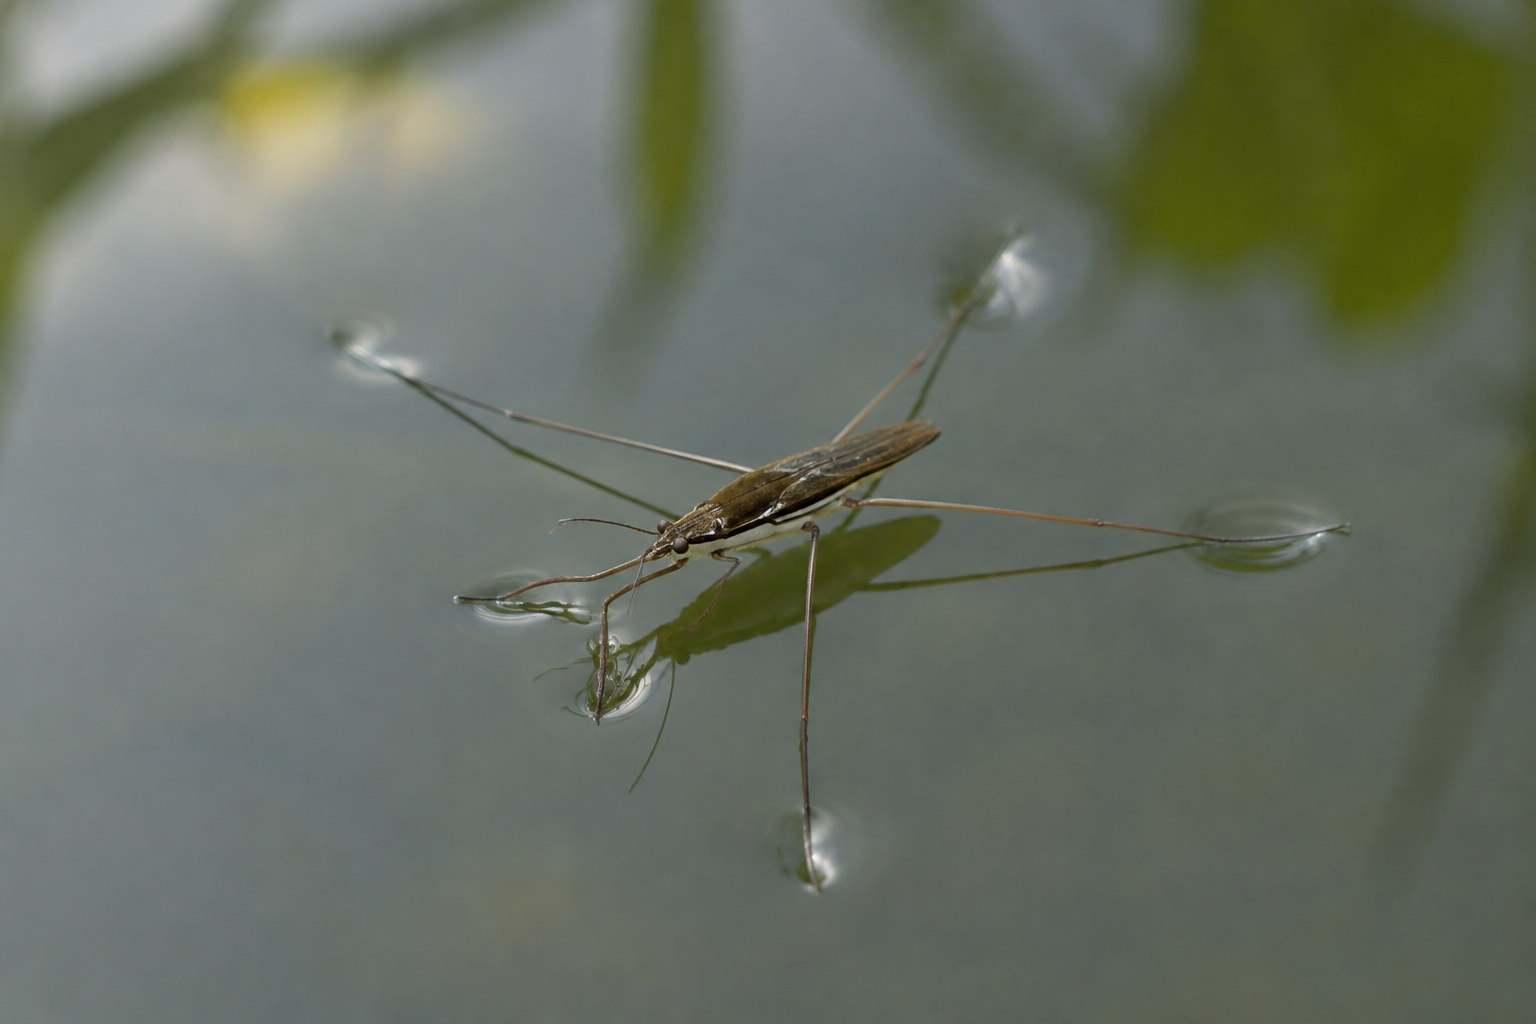
\includegraphics[width=0.6\linewidth]{images/book3/ai/b3-08-water-strider.png}

{\small جوّاب ماء على بركة: والغمازات تحت قوائمه هي السطح المشدود
بتماسك ماء مرتبط \omterm{def:b1:water-small-molecules:water}{بروابط هيدروجينية}.}
\end{omfigure}

\begin{example}[الأثر الكاره للماء في العمل]\label{ex:b1:water-small-molecules:hydrophobic}
رجّ زيتًا في ماء، فتكون القطيرات قد اندمجت في دقائق: إذ يعصر الماء ما
لا يستطيع أن يرتبط به. والأثر نفسه يطوي بروتينًا (فتختبئ بقاياه
الزيتية في الداخل، \cref{ch:b1:proteins})، ويركّب غشاءً (فتتجمع ذيول
الدهون بعيدًا عن الماء، \cref{ch:b1:lipids})، ويدفع سطحين جزيئيين
متوافقين أحدهما إلى الآخر. فلا شيء يجذب الزيت إلى الزيت؛ بل الماء
يدفع.
\end{example}

\section{الروابط الضعيفة}

\begin{definition}[الروابط التساهمية وغير التساهمية]\label{def:b1:water-small-molecules:bonds}
\emph{الرابطة التساهمية}\index{رابطة تساهمية} تتقاسم زوجًا
إلكترونيًا بين ذرتين وتكلف \qtyrange{300}{500}{kJ/mol} لكسرها: فهياكل
الجزيئات تساهمية، ولا يعقدها في \omterm{def:b1:cell-unit-of-life:cell}{الخلية} أو يكسرها إلا الإنزيمات.
أما \emph{الروابط غير التساهمية}\index{رابطة غير تساهمية} فهي
التجاذبات الضعيفة العكوسة التي تمسك الجزيئات \emph{بعضها ببعض} وتشكلها:
\emph{\omterm{def:b1:water-small-molecules:water}{الرابطة الهيدروجينية}} (\qtyrange{4}{20}{kJ/mol} في الماء)؛
و\emph{الرابطة الشاردية}\index{رابطة شاردية} بين شحنتين متعاكستين
(نحو \qty{12}{kJ/mol} في الماء، وثابته العازل يحجب الشحنات ثمانين
ضعفًا)؛ وتجاذبات \emph{فان دير فالس}\index{قوة فان دير فالس} بين أي
ذرتين متلامستين (\qtyrange{1}{4}{kJ/mol} لكل منها، لكنها تُجمع على
سطح كامل)؛ و\emph{\omterm{prop:b1:water-small-molecules:properties}{الأثر الكاره للماء}}، وهو ليس رابطة بل استبعاد
الماء للسطوح غير القطبية.
\end{definition}

\begin{proposition}[لماذا كانت الروابط الضعيفة روابط البيولوجيا]\label{prop:b1:water-small-molecules:weak}
الطاقة الحرارية عند \qty{37}{\celsius} هي $RT = \qty{2.6}{kJ/mol}$.
والرابطة الضعيفة الواحدة ليست إلا بضعة أمثال ذلك وتنكسر في
ميكروثوان؛ أما عشر روابط معًا، على سطحين متوافقين، فتمسك ساعات.
و\emph{التعرف}\index{التعرف الجزيئي} الجزيئي --- إنزيم لركيزته، وضد
مناعي لمولد ضده، وخصلة DNA لمتممتها --- يقوم على روابط ضعيفة كثيرة
تُعقد دفعة واحدة بين سطحين متكاملين، ولهذا كان في آن نوعيًا (فلا
يعقدها كلها إلا سطح موافق) وعكوسًا (فالحرارة أو منافس ينقضه). أما
الروابط التساهمية، وهي أقوى بمئة مرة، فكانت لتكون دائمة.
\end{proposition}

\begin{example}[إذابة لولب مزدوج]\label{ex:b1:water-small-molecules:melting}
تمسك خصلتي DNA رابطتان أو ثلاث \omterm{def:b1:water-small-molecules:water}{روابط هيدروجينية} لكل زوج قواعد، مع
تكديس (\omterm{def:b1:water-small-molecules:bonds}{فان دير فالس}) الأزواج المتجاورة؛ وزوج واحد كان لينفصل في
الحال، لكن ألف زوج متتابع تمسك حتى تبلغ الحرارة نحو
\qty{90}{\celsius}، ثم تلتئم، بالتقابل نفسه بالضبط، حين تُخفض
(\cref{ch:b1:nucleic-acids}). نوعية، وقوية بالعدد، وعكوسة.
\end{example}

\section{الحموض والأسس والهوادئ}

\begin{definition}[pH والحمض والأساس وp$K_a$]\label{def:b1:water-small-molecules:ph}
ينفصل الماء انفصالًا طفيفًا، $\mathrm{H_2O} \rightleftharpoons
\mathrm{H^+} + \mathrm{OH^-}$، مع $[\mathrm{H^+}][\mathrm{OH^-}] =
K_w = \qty{e-14}{mol^2/L^2}$ عند \qty{25}{\celsius}. و\emph{pH}\index{pH}
هو $-\log_{10}[\mathrm{H^+}]$: أي 7 للماء النقي، وأدنى للحموض، وأعلى
للأسس. و\emph{الحمض}\index{حمض} $\mathrm{HA}$ يطلق بروتونًا،
$\mathrm{HA} \rightleftharpoons \mathrm{H^+} +
\mathrm{A^-}$، بثابت
انفصال $K_a =
[\mathrm{H^+}][\mathrm{A^-}]/[\mathrm{HA}]$
و\emph{p$K_a$}\index{pKa@p$K_a$} $= -\log_{10}K_a$؛ وأساسه
\emph{المرافق}\index{أساس} $\mathrm{A^-}$ يقبل بروتونًا. والحمض القوي
(HCl) منفصل انفصالًا تامًا؛ أما حموض \omterm{def:b1:cell-unit-of-life:cell}{الخلية} (الحموض الكربوكسيلية،
والفوسفات، والأمونيوم) فضعيفة، وp$K_a$ لها بين 2 و10.
\end{definition}

\begin{theorem}[هندرسون--هاسلبالخ]\label{thm:b1:water-small-molecules:hh}
\index{معادلة هندرسون--هاسلبالخ}
من أجل \omterm{def:b1:water-small-molecules:ph}{حمض} ضعيف في محلول،
\[
\mathrm{pH} = \mathrm{p}K_a + \log_{10}\frac{[\mathrm{A^-}]}{[\mathrm{HA}]} .
\]
وعند $\mathrm{pH} = \mathrm{p}K_a$ يكون \omterm{def:b1:water-small-molecules:ph}{الحمض} منفصلًا بنصفه؛ وفوق
ذلك بوحدة \omterm{def:b1:water-small-molecules:ph}{pH} واحدة يكون منفصلًا \qty{91}{\%}؛ ودونها \qty{9}{\%}.
\end{theorem}
\begin{proof}
خذ لوغاريتم $K_a = [\mathrm{H^+}][\mathrm{A^-}]/[\mathrm{HA}]$:
$\log K_a = \log[\mathrm{H^+}] + \log([\mathrm{A^-}]/[\mathrm{HA}])$،
أي $-\mathrm{p}K_a = -\mathrm{pH} + \log([\mathrm{A^-}]/[\mathrm{HA}])$.
والنسبة $1$ و$10$ و$0.1$ عند \omterm{def:b1:water-small-molecules:ph}{pH} $= \mathrm{p}K_a$ و$\mathrm{p}K_a + 1$
و$\mathrm{p}K_a - 1$.
\end{proof}

\begin{definition}[الهادئة]\label{def:b1:water-small-molecules:buffer}
\emph{الهادئة}\index{هادئة} محلول يحوي حمضًا ضعيفًا وأساسه \omterm{def:b1:water-small-molecules:ph}{المرافق}
بمقادير متقاربة؛ وهو يقاوم تغير \omterm{def:b1:water-small-molecules:ph}{pH}، لأن ما يُضاف من $\mathrm{H^+}$
يأخذه $\mathrm{A^-}$ وما يُضاف من $\mathrm{OH^-}$ يأخذه
$\mathrm{HA}$. وهي تعمل أحسن ما تعمل في حدود وحدة واحدة من
p$K_a$، وتنمو \emph{سعتها} مع مجموع تركيز الزوج. وهوادئ \omterm{def:b1:cell-unit-of-life:cell}{الخلية} هي:
الفوسفات ($\mathrm{H_2PO_4^-}/\mathrm{HPO_4^{2-}}$، وp$K_a$ لها 6.8)
والسلاسل الجانبية للبروتينات داخل \omterm{def:b1:cell-unit-of-life:cell}{الخلايا}؛ والبيكربونات
($\mathrm{CO_2}/\mathrm{HCO_3^-}$، وp$K_a$ فعالة 6.1) في الدم،
وشريكها الحمضي غاز تستطيع الرئتان إزالته.
\end{definition}

\begin{omfigure}
\begin{tikzpicture}
\begin{axis}[
  width=0.86\linewidth, height=6.2cm,
  axis x line=bottom, axis y line=left,
  xmin=0, xmax=1, ymin=3, ymax=11,
  xlabel={كسر الحمض المعادَل (مكافئات $\mathrm{OH^-}$ المضافة)}, ylabel={pH},
  xlabel style={font=\small, at={(axis description cs:0.5,-0.12)}, anchor=north},
  ylabel style={font=\small},
  tick label style={font=\small}, xtick={0,0.25,0.5,0.75,1}, ytick={3,4,5,6,7,8,9,10,11},
  clip=false,
]
\addplot[very thick, omDef, domain=0.02:0.98, samples=120] {6.8 + log10(x/(1-x))};
\draw[dashed, gray] (axis cs:0,6.8) -- (axis cs:0.5,6.8);
\draw[dashed, gray] (axis cs:0.5,3) -- (axis cs:0.5,6.8);
\node[font=\scriptsize, anchor=south west] at (axis cs:0.02,6.85) {pH $=$ p$K_a$ $= 6.8$ عند نصف المعادلة};
\draw[<->, thick, omThm] (axis cs:0.09,5.8) -- (axis cs:0.91,7.8);
\node[font=\scriptsize, omThm, anchor=north west, align=left] at (axis cs:0.55,5.7) {مدى الهدأة:\\ p$K_a \pm 1$، منحنٍ مستو};
\end{axis}
\end{tikzpicture}

{\small معايرة \omterm{def:b1:water-small-molecules:ph}{حمض} ضعيف (الفوسفات، وp$K_a$ لها 6.8) \omterm{def:b1:water-small-molecules:ph}{بأساس}. والمنحني
مستوٍ حول p$K_a$: فهناك تغير إضافة \omterm{def:b1:water-small-molecules:ph}{الأساس} نسبة \omterm{def:b1:water-small-molecules:ph}{الأساس} إلى \omterm{def:b1:water-small-molecules:ph}{الحمض} ولا
تكاد تغير \omterm{def:b1:water-small-molecules:ph}{pH}. وخارج المدى ينساح \omterm{def:b1:water-small-molecules:ph}{pH} بحرية.}
\end{omfigure}

\begin{omfigure}
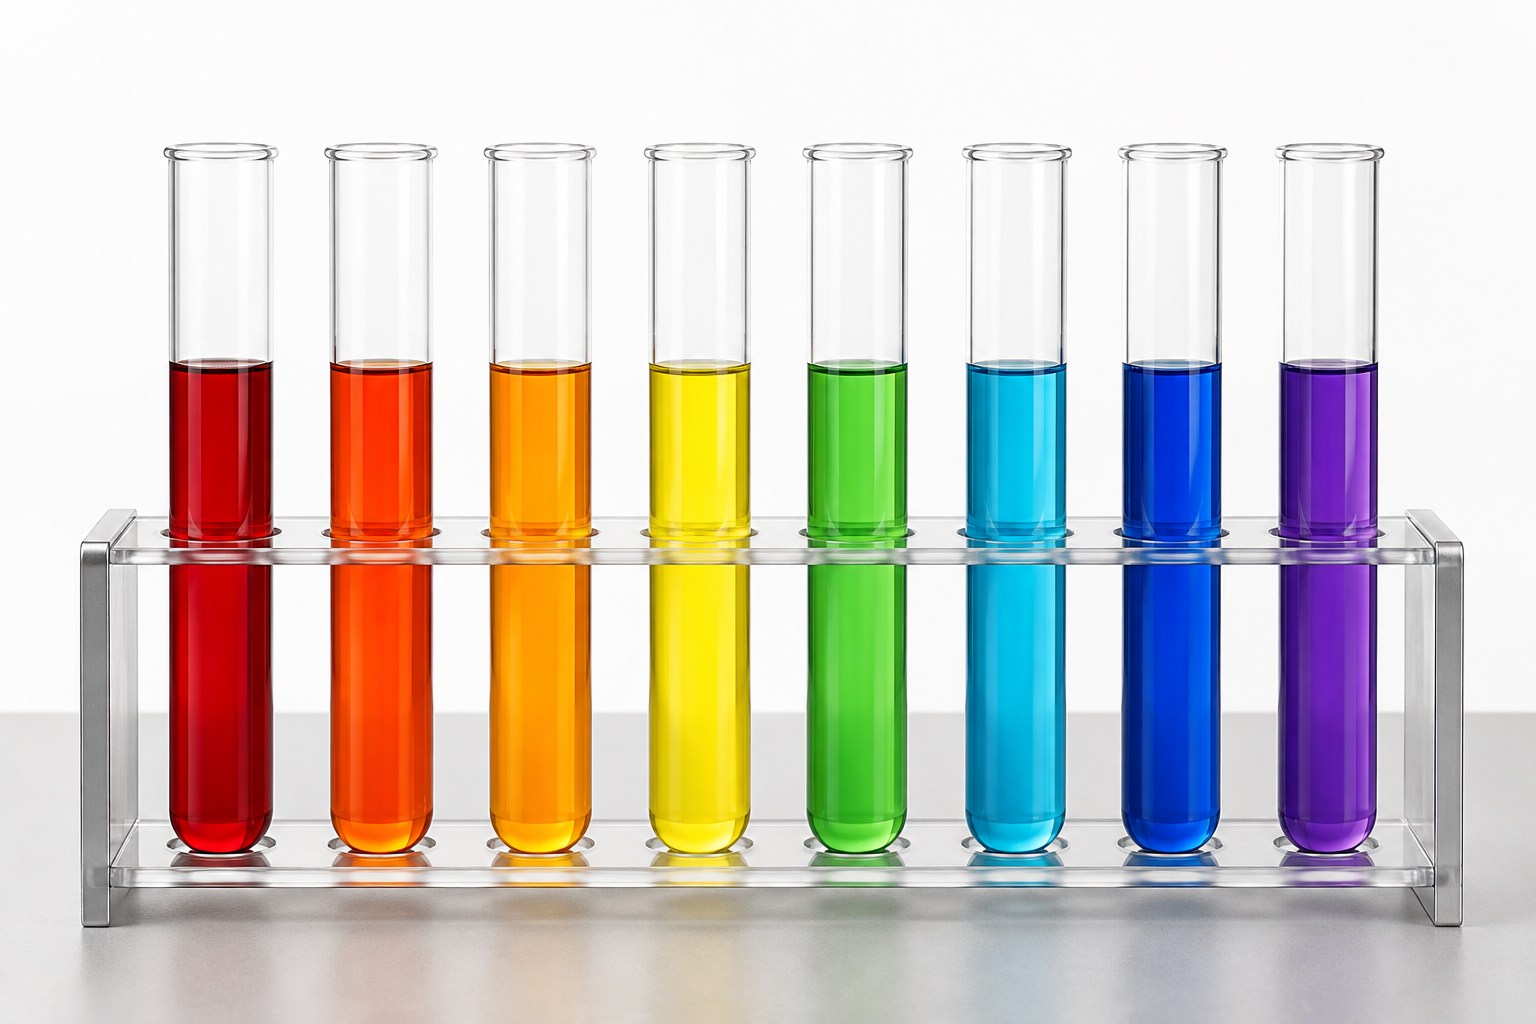
\includegraphics[width=0.6\linewidth]{images/book3/ai/b3-08-indicator-tubes.png}

{\small سلم \omterm{def:b1:water-small-molecules:ph}{pH} منظورًا بكاشف عام: من الأحمر عند \omterm{def:b1:water-small-molecules:ph}{pH} 2 إلى البنفسجي عند
\omterm{def:b1:water-small-molecules:ph}{pH} 12. فالعصارة المعدية عند 1--2، والبول 5--8، والدم 7.4، والمعي
الدقيق 8، \omterm{def:b1:eukaryotic-cell:organelle}{والعصارة الخلوية} 7.2، \omterm{def:b1:eukaryotic-cell:endomembrane}{والجسيم الحال} 5، ولمعة الثايلاكويد في
الضوء 5، والسدى 8.}
\end{omfigure}

\begin{method}[حساب الهوادئ]\label{met:b1:water-small-molecules:bufferarith}
\begin{enumerate}
  \item عيّن زوج \omterm{def:b1:water-small-molecules:ph}{الحمض} \omterm{def:b1:water-small-molecules:ph}{والأساس} وp$K_a$ له عند حرارة العمل.
  \item طبّق هندرسون--هاسلبالخ لتحصل على نسبة \omterm{def:b1:water-small-molecules:ph}{الأساس} إلى \omterm{def:b1:water-small-molecules:ph}{الحمض} من
        \omterm{def:b1:water-small-molecules:ph}{pH}، أو على \omterm{def:b1:water-small-molecules:ph}{pH} من التراكيز.
  \item لإضافة \omterm{def:b1:water-small-molecules:ph}{حمض} قوي: اطرح مقداره من \omterm{def:b1:water-small-molecules:ph}{الأساس} وأضفه إلى \omterm{def:b1:water-small-molecules:ph}{الحمض}، ثم أعد
        حساب \omterm{def:b1:water-small-molecules:ph}{pH}. ولإضافة \omterm{def:b1:water-small-molecules:ph}{أساس} قوي: العكس.
  \item وإذا كان أحد الشريكين يستطيع مغادرة الجملة (ثاني أكسيد كربون
        يُزفر، أو أمونياك يُطرح)، فالجملة \emph{مفتوحة}: أبقِ ذلك
        الشريك عند قيمته المفروضة بدل أن تدعه يتراكم. والهوادئ
        المفتوحة تحفظ \omterm{def:b1:water-small-molecules:ph}{pH} أحسن بكثير من المغلقة.
\end{enumerate}
\end{method}

\begin{example}[الدم]\label{ex:b1:water-small-molecules:blood}
يحمل الدم الشرياني \qty{24}{mmol/L} من البيكربونات و$\mathrm{CO_2}$
منحلًا عند \qty{1.2}{mmol/L} (تضبطه الرئتان):
$\mathrm{pH} =
6.1 + \log(24/1.2) = 6.1 + 1.30 = 7.4$. وإضافة
\qty{5}{mmol/L} من \omterm{def:b1:water-small-molecules:ph}{حمض} تحول \qty{5}{mmol/L} من البيكربونات إلى
$\mathrm{CO_2}$؛ فإن نفثت الرئتان ذلك $\mathrm{CO_2}$ وأبقتا القيمة
المنحلة، صار \omterm{def:b1:water-small-molecules:ph}{pH} يساوي $6.1 + \log(19/1.2) = 7.30$؛ أما في دورق مغلق
فكان $\mathrm{CO_2}$ ليرتفع إلى \qty{6.2}{mmol/L} ويهبط \omterm{def:b1:water-small-molecules:ph}{pH} إلى
$6.1 + \log(19/6.2) =
6.59$. فالرئتان هما الفارق.
\end{example}

\section{الجزيئات الحيوية الصغيرة}

\begin{definition}[الزمر الوظيفية]\label{def:b1:water-small-molecules:groups}
الجزيئات العضوية في \omterm{def:b1:cell-unit-of-life:cell}{الخلية} هياكل كربونية تحمل مجموعة صغيرة من
\emph{الزمر الوظيفية}\index{زمرة وظيفية} تحدد كيمياءها:
\begin{center}
\small
\begin{tabular}{llll}
\hline
الزمرة & الصيغة & الخاصية & توجد في \\
\hline
هيدروكسيل & $-\mathrm{OH}$ & قطبية، تعقد \omterm{def:b1:water-small-molecules:water}{روابط هيدروجينية} & السكريات، الكحولات \\
كربونيل & $>\!\mathrm{C{=}O}$ & قطبية، فعالة & الألدوزات، الكيتوزات \\
كربوكسيل & $-\mathrm{COOH}$ & حمضية (p$K_a \approx 4$) & الحموض الدسمة، الحموض الأمينية \\
أميني & $-\mathrm{NH_2}$ & أساسية (p$K_a \approx 9$) & الحموض الأمينية \\
فوسفات & $-\mathrm{OPO_3^{2-}}$ & مشحونة، روابط غنية بالطاقة & النوكليوتيدات، \omterm{def:b1:water-small-molecules:atp}{ATP} \\
سلفهيدريل & $-\mathrm{SH}$ & تعقد جسور S--S & السيستئين \\
ميثيل & $-\mathrm{CH_3}$ & غير قطبية & الدهون، وسمات DNA \\
\hline
\end{tabular}
\end{center}
وعند \omterm{def:b1:water-small-molecules:ph}{pH} \omterm{def:b1:cell-unit-of-life:cell}{الخلية} تكون زمر الكربوكسيل مشرَّدة ($-\mathrm{COO^-}$) وزمر
الأمين مبرتنة ($-\mathrm{NH_3^+}$).
\end{definition}

\begin{proposition}[أربع عائلات من لبنات البناء]\label{prop:b1:water-small-molecules:families}
تكاد كل المادة العضوية في \omterm{def:b1:cell-unit-of-life:cell}{الخلية} تُبنى من أربعة أنواع من الجزيئات
الصغيرة، كل منها بضع مئات من الدالتونات: \emph{السكريات}
(\cref{ch:b1:carbohydrates})، و\emph{الحموض الدسمة}
(\cref{ch:b1:lipids})، و\emph{الحموض الأمينية}
(\cref{ch:b1:proteins})، و\emph{النوكليوتيدات}
(\cref{ch:b1:nucleic-acids}). وثلاثة منها تُوصل في \emph{بوليمرات}
--- السكريات المتعددة، والبروتينات، والحموض النووية --- بعملية
\emph{التكاثف}\index{تكاثف} (وهي رابطة تُعقد بفقد جزيء ماء)، وتُفكك
\emph{بالحلمهة}\index{حلمهة} (فتُكسر الرابطة بإضافة ماء). \omterm{prop:b1:water-small-molecules:families}{والتكاثف}
صعودي يدفع ثمنه \omterm{def:b1:water-small-molecules:atp}{ATP}؛ والحلمهة هبوطية لا تحتاج إلا إلى إنزيم.
\end{proposition}

\begin{omfigure}
\begin{tikzpicture}[font=\small, >=Stealth, line cap=round,
  mono/.style={draw, thick, rounded corners=3pt, minimum width=16mm, minimum height=8mm, fill=omDef!12}]
  \node[mono] (a) at (0,0) {وحيدة};
  \node[mono] (b) at (2.4,0) {وحيدة};
  \node[font=\footnotesize] at (1.2,0.55) {$-\mathrm{OH}$ \quad $\mathrm{H}-$};
  \draw[->, very thick, omExo] (3.6,0.15) -- (5.6,0.15) node[midway, above, font=\footnotesize, align=center] {تكاثف\\ (يُدفع ثمنه ATP)};
  \draw[->, very thick, omThm] (5.6,-0.15) -- (3.6,-0.15) node[midway, below, font=\footnotesize, align=center] {حلمهة\\ (إنزيم فقط)};
  \node[mono, minimum width=34mm] (ab) at (7.6,0) {وحيدة---وحيدة};
  \node[font=\footnotesize] at (7.6,0.55) {رابطة تساهمية};
  \node[font=\footnotesize, omDef] at (9.9,-0.6) {$+\ \mathrm{H_2O}$};
\end{tikzpicture}

{\small \omterm{prop:b1:water-small-molecules:families}{التكاثف} يصل لبنتي بناء بفقد جزيء ماء؛ والحلمهة تفككهما بإضافة
جزيء ماء. وهكذا تُبلمر السكريات والحموض الأمينية والنوكليوتيدات.}
\end{omfigure}

\begin{example}[جرد الخلية]\label{ex:b1:water-small-molecules:inventory}
من الكتلة الجافة لبكتيريا، تكون البروتينات \qty{55}{\%}، وRNA
\qty{20}{\%}، وDNA \qty{3}{\%}، والدهون \qty{9}{\%}، والسكريات
المتعددة \qty{5}{\%}، والباقي جزيئات صغيرة وشوارد. أما بعدد الجزيئات
فتنقلب الصورة: ألف نوع من المستقلبات الصغيرة والشوارد، بتراكيز من
النانومول إلى عُشر المول في اللتر، تكوّن معظم الجزيئات التي ليست ماءً.
فالبوتاسيوم عند \qty{150}{mmol/L}، والغلوتامات \qty{100}{mmol/L}،
\omterm{def:b1:water-small-molecules:atp}{وATP} \qty{5}{mmol/L}، وعامل استنساخ عند بضعة جزيئات في \omterm{def:b1:cell-unit-of-life:cell}{الخلية}.
\end{example}

\section{الطاقة: الطاقة الحرة وATP}

\begin{proposition}[الطاقة الحرة لتفاعل]\label{prop:b1:water-small-molecules:gibbs}
\index{الطاقة الحرة}
يجري التفاعل عند حرارة وضغط ثابتين تلقائيًا في الاتجاه الذي يخفض
طاقة غيبس الحرة $G$. فمن أجل
$\mathrm{A} + \mathrm{B} \rightleftharpoons \mathrm{C} + \mathrm{D}$،
\[
\Delta G = \Delta G^{\circ\prime} + RT\ln\frac{[\mathrm{C}][\mathrm{D}]}{[\mathrm{A}][\mathrm{B}]},
\]
حيث $\Delta G^{\circ\prime}$ هو تغير \omterm{prop:b1:water-small-molecules:gibbs}{الطاقة الحرة} المعياري (بكل
التراكيز \qty{1}{mol/L} وعند \omterm{def:b1:water-small-molecules:ph}{pH} 7) والحد اللوغاريتمي يصحح للتراكيز
الفعلية. وعند التوازن يكون $\Delta G = 0$، فيكون
$\Delta G^{\circ\prime} = -RT\ln K'_{\text{توازن}}$: فكل
\qty{5.7}{kJ/mol} من $\Delta G^{\circ\prime}$ تزيح ثابت التوازن عشرة
أضعاف. و$\Delta G$ يقول إلى أي جهة يستطيع التفاعل أن يجري، لا بأي
سرعة: فتلك شأن الإنزيم (\cref{ch:b1:enzymes}).
\end{proposition}
\begin{proof}
الكمون الكيميائي لكل نوع هو $\mu = \mu^\circ + RT\ln c$ (وهي نتيجة
المحلول المثالي في مقرر الفيزياء)؛ و$\Delta G$ مجموع كمونات النواتج
ناقص كمونات المتفاعلات، وهذا يعطي الصيغة؛ وجعله صفرًا عند التوازن
يعطي العلاقة مع $K'_{\text{توازن}}$.
\end{proof}

\begin{definition}[ATP والاقتران]\label{def:b1:water-small-molecules:atp}
\emph{ATP}\index{ATP} (أدينوزين ثلاثي الفوسفات) نوكليوتيد
(\cref{ch:b1:nucleic-acids}) يحمل ثلاث فوسفات متتابعة؛ والرابطتان
الخارجيتان \emph{فوسفوأنهيدريديتان}\index{رابطة فوسفوأنهيدريدية}،
وحلمهتهما، $\mathrm{ATP} + \mathrm{H_2O} \to \mathrm{ADP} +
\mathrm{P_i}$، لها $\Delta G^{\circ\prime} = \qty{-30.5}{kJ/mol}$،
وعند تراكيز \omterm{def:b1:cell-unit-of-life:cell}{الخلية} $\Delta G \approx \qty{-50}{kJ/mol}$. وATP هو
\emph{عملة الطاقة}\index{عملة الطاقة} في \omterm{def:b1:cell-unit-of-life:cell}{الخلية}: فالهدم يصنعه
(\cref{ch:b1:respiration-fermentation})، والتركيب الحيوي والنقل
والحركة تنفقه. ويُجعل التفاعل الصعودي يجري \emph{باقترانه}\index{اقتران الطاقة}
بحلمهة ATP عبر وسيط مشترك، حتى يكون مجموع $\Delta G$ للتفاعلين سالبًا.
\end{definition}

\begin{example}[لماذا تحرر حلمهة ATP هذا القدر]\label{ex:b1:water-small-molecules:whyatp}
ثلاثة أسباب: الشحنات السالبة الأربع لفوسفات \omterm{def:b1:water-small-molecules:atp}{ATP} يتنافر بعضها مع بعض
ويزول تنافرها بالشطر؛ والناتجان $\mathrm{ADP}$ و$\mathrm{P_i}$ أكثر
استقرارًا بالرنين وبالإماهة من الأنهيدريد؛ \omterm{def:b1:cell-unit-of-life:cell}{والخلية} تبقي \omterm{def:b1:water-small-molecules:atp}{ATP} فوق
توازنه مع ADP والفوسفات بألف مرة. والأخير هو الحد الأكبر: فمع \omterm{def:b1:water-small-molecules:atp}{ATP} عند
\qty{5}{mmol/L} وADP \qty{1}{mmol/L} و$\mathrm{P_i}$
\qty{10}{mmol/L} يكون
$\Delta G = -30.5 + 2.58\ln\frac{10^{-3}\times 10^{-2}}{5\times 10^{-3}}
= -30.5 - 16 = \qty{-46.5}{kJ/mol}$.
\end{example}

\begin{example}[الاقتران]\label{ex:b1:water-small-molecules:coupling}
تفاعل الغلوكوز $+\ \mathrm{P_i} \to$ غلوكوز-6-فوسفات
$+\ \mathrm{H_2O}$ له $\Delta G^{\circ\prime} = \qty{+13.8}{kJ/mol}$:
فعند التوازن لا يكاد أي غلوكوز يُفسفَر. أما الهكسوكيناز فينقل
الفوسفات مباشرة من \omterm{def:b1:water-small-molecules:atp}{ATP}: غلوكوز $+$ \omterm{def:b1:water-small-molecules:atp}{ATP} $\to$ غلوكوز-6-فوسفات $+$
ADP، و$\Delta G^{\circ\prime} = 13.8 - 30.5 =
\qty{-16.7}{kJ/mol}$،
وثابت التوازن $800$، والتفاعل تام عمليًا. والفوسفات لا يظهر حرًا قط:
فالتفاعلان تفاعل واحد.
\end{example}

\section{تمارين}

\begin{exercise}[$\star$]\label{exo:b1:water-small-molecules:1}
فسّر، انطلاقًا من بنية جزيء الماء، لماذا كان الماء مذيبًا حسنًا
للأملاح ورديئًا للزيوت.
\end{exercise}

\begin{exercise}[$\star$]\label{exo:b1:water-small-molecules:2}
رتب أنواع التآثر غير التساهمي الأربعة بحسب القوة وأعطِ دورًا
بيولوجيًا واحدًا لكل منها.
\end{exercise}

\begin{exercise}[$\star$]\label{exo:b1:water-small-molecules:3}
احسب \omterm{def:b1:water-small-molecules:ph}{pH} محلول فيه $[\mathrm{H^+}] = \qty{4e-8}{mol/L}$، ثم
$[\mathrm{H^+}]$ في العصارة المعدية عند \omterm{def:b1:water-small-molecules:ph}{pH} 1.5.
\end{exercise}

\begin{exercise}[$\star$]\label{exo:b1:water-small-molecules:4}
من شكل المعايرة، على أي مدى من \omterm{def:b1:water-small-molecules:ph}{pH} تعمل \omterm{def:b1:water-small-molecules:buffer}{هادئة} الفوسفات، وما نسبة
\omterm{def:b1:water-small-molecules:ph}{الأساس} إلى \omterm{def:b1:water-small-molecules:ph}{الحمض} عند \omterm{def:b1:water-small-molecules:ph}{pH} 7.4؟
\end{exercise}

\begin{exercise}[$\star\star$]\label{exo:b1:water-small-molecules:5}
\omterm{def:b1:water-small-molecules:ph}{لحمض} الخل p$K_a$ يساوي 4.76. فأي كسر منه مشرَّد عند \omterm{def:b1:water-small-molecules:ph}{pH} 4.76، وعند
\omterm{def:b1:water-small-molecules:ph}{pH} 7.2 (\omterm{def:b1:eukaryotic-cell:organelle}{العصارة الخلوية})، وعند \omterm{def:b1:water-small-molecules:ph}{pH} 2 (المعدة)؟ وأي الصورتين تعبر
غشاءً أسهل، وأين يُمتص \omterm{def:b1:water-small-molecules:ph}{حمض} الخل؟
\end{exercise}

\begin{exercise}[$\star\star$]\label{exo:b1:water-small-molecules:6}
\omterm{def:b1:water-small-molecules:buffer}{هادئة} تحوي \qty{50}{mmol/L} من $\mathrm{HPO_4^{2-}}$
و\qty{50}{mmol/L} من $\mathrm{H_2PO_4^-}$ (وp$K_a$ لها 6.8). احسب
\omterm{def:b1:water-small-molecules:ph}{pH} لها. ثم احسب \omterm{def:b1:water-small-molecules:ph}{pH} بعد إضافة \qty{10}{mmol/L} من HCl، وبعد إضافة
HCl نفسه إلى ماء نقي.
\end{exercise}

\begin{exercise}[$\star\star$]\label{exo:b1:water-small-molecules:7}
تبخر العرق يبرّد عدّاءً. فكم عرقًا يجب أن يتبخر لنزع \qty{500}{kJ}؟
وفسّر، \omterm{def:b1:water-small-molecules:water}{بالروابط الهيدروجينية}، لماذا كانت حرارة تبخر الماء كبيرة إلى
هذا الحد.
\end{exercise}

\begin{exercise}[$\star\star$]\label{exo:b1:water-small-molecules:8}
تفاعل غلوكوز-1-فوسفات $\to$ غلوكوز-6-فوسفات له
$K'_{\text{توازن}} = 19$ عند \qty{25}{\celsius}. احسب
$\Delta G^{\circ\prime}$. وفي \omterm{def:b1:cell-unit-of-life:cell}{خلية} يكون فيها غلوكوز-6-فوسفات عند
\qty{2}{mmol/L} وغلوكوز-1-فوسفات عند \qty{0.02}{mmol/L}، احسب
$\Delta G$ وقل إلى أي جهة يجري التفاعل.
\end{exercise}

\begin{exercise}[$\star\star$]\label{exo:b1:water-small-molecules:9}
لماذا تتجمد بحيرة من أعلى إلى أسفل، ولماذا يهم هذا السمك الذي فيها؟
وماذا كان ليحدث في عالم يغوص فيه الجليد؟
\end{exercise}

\begin{exercise}[$\star\star\star$]\label{exo:b1:water-small-molecules:10}
احسب $\Delta G$ لحلمهة \omterm{def:b1:water-small-molecules:atp}{ATP} في \omterm{def:b1:cell-unit-of-life:cell}{خلية} عضلية يكون فيها \omterm{def:b1:water-small-molecules:atp}{ATP} عند
\qty{8}{mmol/L} وADP \qty{0.9}{mmol/L} و$\mathrm{P_i}$
\qty{8}{mmol/L} عند \qty{37}{\celsius}؛ ثم في عضلة متعبة يكون فيها
\omterm{def:b1:water-small-molecules:atp}{ATP} عند \qty{5}{mmol/L} وADP \qty{3}{mmol/L} و$\mathrm{P_i}$
\qty{30}{mmol/L}. فماذا فعل التعب بالطاقة المتاحة لكل \omterm{def:b1:water-small-molecules:atp}{ATP}؟
\end{exercise}

\begin{exercise}[$\star\star\star$]\label{exo:b1:water-small-molecules:11}
\omterm{def:b1:cell-unit-of-life:cell}{خلية} عند \omterm{def:b1:water-small-molecules:ph}{pH} 7.2 و\qty{37}{\celsius} حجمها الداخلي
\qty{1000}{\micro m^3}. فكم شاردة $\mathrm{H^+}$ حرة تحوي؟ قارن مع
زمرها \omterm{def:b1:water-small-molecules:buffer}{الهادئة} البالغة $\num{3e9}$. وماذا تقول المقارنة عن معنى
«\omterm{def:b1:water-small-molecules:ph}{pH} \omterm{def:b1:cell-unit-of-life:cell}{الخلية}»؟
\end{exercise}

\begin{exercise}[$\star\star\star$]\label{exo:b1:water-small-molecules:12}
«الحياة طريقة في إبقاء التفاعلات بعيدة عن التوازن.» ناقش في فقرة،
مستعملًا نسبة تركيز \omterm{def:b1:water-small-molecules:atp}{ATP}، والاقتران، وما يحل \omterm{def:b1:cell-unit-of-life:cell}{بخلية} يبلغ \omterm{def:b1:water-small-molecules:atp}{ATP} فيها
توازنه مع ADP.
\end{exercise}

\section{مسألة: الدم هادئةً}

\begin{problem}[{مسألة نهاية الأسبوع --- خمسة لترات من الدم عند pH 7.40
خلال عدو سريع: البيكربونات، وثاني أكسيد الكربون، والرئتان،
والكليتان، وصولًا إلى إزاحة pH من أجل حمل لاكتات معطى}]
\label{pb:b1:water-small-molecules:1}
الدم الشرياني: \omterm{def:b1:water-small-molecules:ph}{pH} 7.40، والبيكربونات
$[\mathrm{HCO_3^-}] =
\qty{24}{mmol/L}$، وثاني أكسيد الكربون المنحل
$[\mathrm{CO_2}] =
\qty{1.2}{mmol/L}$ (وهو متناسب مع ضغطه الجزئي:
فضغط جزئي قدره \qty{40}{mmHg} يعطي \qty{1.2}{mmol/L}). ولجملة
البيكربونات p$K_a$ فعالة قدرها 6.1: $\mathrm{CO_2} + \mathrm{H_2O}
\rightleftharpoons \mathrm{H^+} + \mathrm{HCO_3^-}$. وحجم الدم
\qty{5}{L}. وبروتينات البلازما والهيموغلوبين تضيف \omterm{def:b1:water-small-molecules:buffer}{هادئة} ثانية سعتها
\qty{25}{mmol} من $\mathrm{H^+}$ لكل لتر لكل وحدة \omterm{def:b1:water-small-molecules:ph}{pH}. والعدو السريع
يطلق \qty{60}{mmol} من \omterm{def:b1:water-small-molecules:ph}{حمض} اللبن (وهو \omterm{def:b1:water-small-molecules:ph}{حمض} قوي عند \omterm{def:b1:water-small-molecules:ph}{pH} الدم) في الدم
خلال دقيقة.

\medskip
\noindent\textbf{الجزء الأول --- حالة الراحة.}
\begin{enumerate}
  \item تحقق من \omterm{def:b1:water-small-molecules:ph}{pH} الدم الشرياني من قيمتي البيكربونات وثاني أكسيد
        الكربون.
  \item احسب $[\mathrm{H^+}]$ عند \omterm{def:b1:water-small-molecules:ph}{pH} 7.40، بالنانومول في اللتر.
  \item كم بروتونًا حرًا في حجم الدم كله؟ قارن مع \qty{120}{mmol} من
        البيكربونات.
  \item احسب نسبة البيكربونات إلى ثاني أكسيد الكربون المنحل والكسر من
        زوج \omterm{def:b1:water-small-molecules:buffer}{الهادئة} الموجود أساسًا.
  \item للدم الوريدي ضغط جزئي من $\mathrm{CO_2}$ قدره \qty{46}{mmHg}
        و\qty{25}{mmol/L} من البيكربونات. احسب \omterm{def:b1:water-small-molecules:ph}{pH} له.
  \item لماذا لم تكن p$K_a$ البالغة 6.1، وهي أدنى من \omterm{def:b1:water-small-molecules:ph}{pH} الدم بأكثر من
        وحدة، عائقًا لهذه \omterm{def:b1:water-small-molecules:buffer}{الهادئة} في الجسم، مع أنها كانت لتكون عائقًا
        في دورق؟
\end{enumerate}

\medskip
\noindent\textbf{الجزء الثاني --- العدو، جملة مغلقة.}
افترض أولًا أن ثاني أكسيد الكربون لا يستطيع المغادرة: فكل بروتون
تأخذه البيكربونات يصير $\mathrm{CO_2}$ منحلًا.
\begin{enumerate}[resume]
  \item احسب تركيز \omterm{def:b1:water-small-molecules:ph}{حمض} اللبن المضاف إلى الدم.
  \item احسب البيكربونات الجديدة و$\mathrm{CO_2}$ المنحل الجديد إذا
        هدأت البيكربونات \omterm{def:b1:water-small-molecules:ph}{الحمض} كله.
  \item احسب \omterm{def:b1:water-small-molecules:ph}{pH} الناتج.
  \item احسب \omterm{def:b1:water-small-molecules:ph}{pH} الذي كان \omterm{def:b1:water-small-molecules:ph}{الحمض} نفسه ليعطيه في \qty{5}{L} من الماء
        النقي.
  \item هل جملة البيكربونات المغلقة \omterm{def:b1:water-small-molecules:buffer}{هادئة} جيدة لهذا الحمل؟ قدّر ذلك
        بإزاحة \omterm{def:b1:water-small-molecules:ph}{pH}.
  \item احسب تغير $[\mathrm{H^+}]$ بين \omterm{def:b1:water-small-molecules:ph}{pH} 7.40 \omterm{def:b1:water-small-molecules:ph}{وpH} السؤال 9، والكسر
        من البروتونات المضافة الذي يبقى حرًا في المحلول.
\end{enumerate}

\medskip
\noindent\textbf{الجزء الثالث --- العدو، جملة مفتوحة.}
تبقي الرئتان الآن $\mathrm{CO_2}$ المنحل عند \qty{1.2}{mmol/L}
بنفث الفائض.
\begin{enumerate}[resume]
  \item احسب \omterm{def:b1:water-small-molecules:ph}{pH} مع البيكربونات عند قيمتها الجديدة و$\mathrm{CO_2}$
        مثبتًا عند \qty{1.2}{mmol/L}.
  \item كم مليمولًا من $\mathrm{CO_2}$ يجب أن تزيله الرئتان، فوق
        الحصيلة في الراحة، لتثبيت القيمة؟
  \item الحصيلة في الراحة \qty{10}{mmol} من $\mathrm{CO_2}$ في
        الدقيقة. فبأي عامل يجب أن ترتفع التهوية دقيقةً لإزالة الفائض؟
  \item يزيد العدّاء في فرط التهوية، فيدفع الضغط الجزئي
        لغاز $\mathrm{CO_2}$ إلى \qty{30}{mmHg}. احسب $\mathrm{CO_2}$
        المنحل الجديد \omterm{def:b1:water-small-molecules:ph}{وpH}.
  \item أدخل الآن \omterm{def:b1:water-small-molecules:buffer}{هادئة} البروتين: فمن \qty{60}{mmol} من البروتونات،
        تأخذ البروتينات حصة بنسبة سعتي الهادئتين. قدّر سعة جملة
        البيكربونات المفتوحة قرب \omterm{def:b1:water-small-molecules:ph}{pH} 7.4 (أي المليمولات من \omterm{def:b1:water-small-molecules:ph}{الحمض} لكل
        لتر التي تزيح \omterm{def:b1:water-small-molecules:ph}{pH} بوحدة واحدة، من هندرسون--هاسلبالخ
        مع $\mathrm{CO_2}$ مثبتًا) وحصة كل \omterm{def:b1:water-small-molecules:buffer}{هادئة} من البروتونات.
  \item أعد حساب \omterm{def:b1:water-small-molecules:ph}{pH} بعد العدو بالهادئتين معًا.
\end{enumerate}

\medskip
\noindent\textbf{الجزء الرابع --- التعافي، والكلية.}
\begin{enumerate}[resume]
  \item في الساعة التالية يؤكسد الكبد اللاكتات (فيزيل \omterm{def:b1:water-small-molecules:ph}{الحمض}). فماذا
        يحل بالبيكربونات وبقيمة \omterm{def:b1:water-small-molecules:ph}{pH}، والرئتان تبقيان $\mathrm{CO_2}$
        ثابتًا؟
  \item مريض بقصور كلوي يحتبس \qty{60}{mmol} من \omterm{def:b1:water-small-molecules:ph}{الحمض} في اليوم ولا
        يستطيع طرحه. احسب هبوط البيكربونات في اليوم (في جملة مفتوحة)
        \omterm{def:b1:water-small-molecules:ph}{وpH} بعد ثلاثة أيام إن لم تُعوَّض البيكربونات.
  \item مريض بداء رئوي يحتبس $\mathrm{CO_2}$ عند ضغط جزئي قدره
        \qty{60}{mmHg} مع بيكربونات \qty{24}{mmol/L}. احسب \omterm{def:b1:water-small-molecules:ph}{pH}.
        وتستجيب الكليتان على مدى أيام برفع البيكربونات إلى
        \qty{33}{mmol/L}؛ احسب \omterm{def:b1:water-small-molecules:ph}{pH} عندئذ.
  \item فسّر في جملتين لماذا تصحح الرئتان \omterm{def:b1:water-small-molecules:ph}{pH} في دقائق والكليتان في
        أيام، وما الذي تتحكم فيه كل منهما في نسبة هندرسون--هاسلبالخ.
  \item تطرح الكليتان \qty{60}{mmol} من \omterm{def:b1:water-small-molecules:ph}{حمض} اليوم في \qty{1.5}{L} من
        البول عند \omterm{def:b1:water-small-molecules:ph}{pH} 5. احسب البروتونات الحرة في ذلك البول، واستنتج
        كيف يُحمل \omterm{def:b1:water-small-molecules:ph}{الحمض}.
  \item القيء يفقد \qty{100}{mmol} من HCl. تنبأ باتجاه تغير \omterm{def:b1:water-small-molecules:ph}{pH}
        واحسبه في الجملة المفتوحة.
  \item اذكر النتيجة: إزاحة \omterm{def:b1:water-small-molecules:ph}{pH} الدم من أجل حمل لاكتات قدره
        \qty{60}{mmol} في الجملة المغلقة، وفي الجملة المفتوحة
        بالبيكربونات وحدها، ومع إضافة هوادئ البروتين.
\end{enumerate}
\end{problem}
